\chapter{บทนำ}
\label{chapter: introduction}

\begin{verse}
``Adapt or perish, now as ever, is nature's inexorable imperative.'' \\
---H.~G.~Wells 
\end{verse}

\begin{verse}
``ปรับตัว หรือ สูญพันธุ์ เป็นความจำเป็นของธรรมชาติที่ไม่อาจหลีกเลี่ยงได้ ทั้งตอนนี้เฉกเช่นตลอดมา'' 
---เอช จี เวลส์ \\
\end{verse}

วิธี\textit{การเรียนรู้ของเครื่อง}ถูกประยุกต์ใช้อย่างกว้างขวางในวงการธุรกิจ อุตสาหกรรม การทหาร วงการวิทยาศาสตร์ บันเทิง รวมถึงการประยุกต์ใช้ชีวิตประจำวัน
ตัวอย่างเช่น 
ลักษณะงานที่เป็น\textit{การทำเหมืองข้อมูล} การตรวจสอบหารูปแบบการใช้บัตรเครดิตที่ผิดปกติ\cite{DeviEtAl2014a} ซึ่งอาจเนื่องมาจากการที่บัตรถูกขโมยไป
การบริหารการลงทุนทางการเงิน\cite{TanEtAl2011a}
งานแอพพลิเคชั่นที่ไม่สามารถโปรแกรมตรงๆได้ (หรือ ทำได้ยากมาก) เช่น ระบบอ่านลายมือเขียน\cite{LeCunEtAl1990a}
การควบคุมเฮลิคอปเตอร์ไร้นักบิน\cite{CoatesEtAl2009a} 
การควบคุมหุ่นยนต์ที่มีการเครื่องไหวที่ซับซ้อน\cite{AkiyamaEtAl2010a}
การบริหารจัดการทรัพยกรนำ้\cite{CastellettiEtAl2013a}
การปรับตั้งค่าของเวอร์ชัวร์แมชชีน\cite{RaoEtAl2009a}
การพัฒนารถยนต์ที่ขับเคลื่อนได้เองโดยไร้คนขับ\cite{ZhuEtAl2014a}
การติดตามลักษณะโครงสร้างใต้น้ำอัตโนมัติ\cite{MagazzeniEtAl2014a}
การระบุหารังสีแกมม่าจากข้อมูลกล้องโทรทัศน์\cite{BockEtAl2004a}
ระบบตรวจสอบการสั่นสะเทือนของแผ่นดินไหว\cite{RuanoEtAl2014a}
การหารูปแบบในข้อมูลชีวสารสนเทศ\cite{KelchtermansEtAl2014a}
การแปลภาษาอัตโนมัติ\cite{CostaFarrus2014a}
ระบบรู้จำคำพูด\cite{SarikayaEtAl2014a}
ระบบรู้จำความก้าวหน้าของคอร์ดดนตรี\cite{YuElAl2013a}
ใช้กับงานศิลปะ\cite{CuljakEtAl2011a}
กีฬา\cite{HolstJanasson2013a}
ระบบรู้จำใบหน้า\cite{BarnardEtAl2013a}
ระบบตรวจสอบความผิดปกติของสัญญาณคลื่นไฟฟ้าหัวใจ\cite{LiEtAl2012a}
การแยกอีเมล์ที่เป็นสแปม\cite{BlanzieriBryl2008a} 
ระบบแนะนำหนังสือ เพลง วิดีโอ หรือสินค้า\cite{GhazanfarPrugel-Bennett2014a}
การจำแนกหรือระบุหัวข้อสำหรับข้อความ\cite{BleiEtAl2003a}
หรือ แม้แต่เพิ่มประสิทธิภาพของงานของระบบควบคุม ระบบตัดสินใจ ที่ซับซ้อน ระบบควบคุมการระบายอากาศ-เครื่องทำความร้อน--เครื่องปรับอากาศ\cite{AndersonEtAl2004a} 
ระบบควบคุมสินค้าคงคลัง\cite{KatanyukulEtAl2011a, KatanyukulEtAl2012a, Katanyukul2013a, KatanyukulChong2014a} 
ระบบควบคุมการจราจร\cite{ChanlohaEtAl2014a} เป็นต้น 

%\begin{minipage}{5.5in}
{\small
\begin{shaded}
%Data mining, also called knowledge discovery in databases, in computer science, the process of discovering interesting and useful patterns and relationships in large volumes of data. The field combines tools from statistics and artificial intelligence (such as neural networks and machine learning) with database management to analyze large digital collections, known as data sets. Data mining is widely used in business (insurance, banking, retail), science research (astronomy, medicine), and government security (detection of criminals and terrorists).
%
การทำเหมืองข้อมูล (Data Mining) หรือ บางครั้งเรียกว่า การค้นหาความรู้ในฐานข้อมูล (Knowledge Discovery in Databases) หมายถึง กระบวนการค้นหารูปแบบหรือความสัมพันธ์ที่น่าสนใจและมีประโยชน์ในข้อมูลขนาดใหญ่
{\footnotesize (จาก Encyclopedia Britainica \verb|https://global.britannica.com/technology/data-mining| สืบค้น 9 สิงหาคม 2559)}
%
การทำเหมืองข้อมูล เน้นที่การค้นหารูปแบบที่น่าสนใจ 
ซึ่งแม้การทำเหมืองข้อมูลอาจจะใช้เทคนิคที่จัดเป็นวิธีการเรียนรู้ของเครื่อง เช่น การหากฏความสัมพันธ์ (Association Rules) การแบ่งกลุ่มข้อมูล (Cluster Analysis) การจำแนกข้อมูล (Classification) เป็นต้น.
แต่ในทางปฏิบัติ บ่อยครั้งที่ในกระบวนการที่สมบูรณ์ของการทำเหมืองข้อมูลจะต้องอาศัยการทำงานของมนุษย์ เช่น กระบวนการอาจมีการใช้มนุษย์ เพื่อตรวจสอบกลั้นกรองผลลัพธ์ที่ได้จากวิธีการเรียนรู้ของเครื่อง
%ความสัมพันธ์ที่น่าสนใจและมีประโยชน์ จากกฏความสัมพันธ์ที่ค้นพบทั้งหมดโดยการหากฏความสัมพันธ์ด้วยคอมพิวเตอร์
หรือแม้แต่กระบวนการการทำเหมืองข้อมูล อาจใช้เพียงการทำงานของมนุษย์ โดยเขียนภาษาสอบถามจากฐานข้อมูล เพื่อค้นหารูปแบบที่น่าสนใจ โดยไม่ต้องอาศัยวิธีของการเรียนรู้ของเครื่องเลยก็ได้.
%
ในขณะที่มุมมองทั่วไปคือการทำเหมืองข้อมูลใช้วิธีจากการเรียนรู้ของเครื่อง 
การเรียนรู้ของเครื่องเองก็อาจจะถูกสร้างขึ้นได้ 
โดยอาศัยข้อมูลและรูปแบบที่ถูกค้นพบโดยการทำเหมือนข้อมูลได้เช่นกัน
\end{shaded}
}
%\end{minipage}


การเรียนรู้ของเครื่อง (Machine Learning) จัดเป็นศาสตร์แขนงหนึ่งของ\textit{ปัญญาประดิษฐ์}. 
ความสำเร็จที่สำคัญๆในวงการปัญญาประดิษฐ์หลายๆอย่าง ก็อาศัยศาสตร์การเรียนรู้ของเครื่อง เช่น โปรแกรมเล่นเกมส์แบคแกมมอน\cite{TDGammon} และ โปรแกรมเล่นหมากล้อม\cite{SilverEtAl2016a} ที่สามารถเล่นได้ระดับสูงสุดเมื่อเทียบกับมนุษย์ 
หรือ ไอบีเอ็มวัตสันที่สามารถชนะมนุษย์ได้ในเกมส์ตอบคำถามเจ๊บพาดี้\cite{Abu-Mostafa2012a}.
%
ประสิทธิผลของการเรียนรู้ของเครื่องและศักยภาพของศาสตร์นี้ทำให้มีการศึกษาวิจัยอย่างกว้างขวางและกระตือรือร้น.
ศาสตร์และศิลป์ของการเรียนรู้ของเครื่อง จึงมีการพัฒนาอย่างมีนัยสำคัญอย่างต่อเนื่อง. 
%
ดาร์พาหรือองค์การโครงการวิจัยชั้นสูงทางการป้องกันประเทศของสหรัฐอเมริกา
(Defense Advanced Research Projects Agency) 
ซึ่งอยู่เบื้องหลังเทคโนโลยีหลายอย่างที่มีผลกระทบต่อเศรษฐกิจและสังคมของทั่วโลก เช่น เทคโนโลยีอินเตอร์เนต 
ก็ให้ความสำคัญและสนับสนุนการวิจัยและพัฒนาศาสตร์และศิลป์ของเทคโนโลยีการเรียนรู้ของเครื่องอย่างกว้างขวาง 
ดังสะท้อนออกมาจากวิสัยทัศน์ของเคทเธอลีนฟิชเชอร์
% (Kathleen Fisher) แห่งดาร์พา 
ที่กล่าวผ่านเวปไซตของดาร์พา ที่ลงข่าวเมื่อ 19 มี.ค. พ.ศ. 2556 ว่า 
%“Our goal is that future machine learning projects won’t require people to know everything about both the domain of interest and machine learning to build useful machine learning applications. Through new probabilistic programming languages specifically tailored to probabilistic inference, we hope to decisively reduce the current barriers to machine learning and foster a boom in innovation, productivity and effectiveness.”
เป้าหมายของดาร์พาคือโครงการ\textit{การเรียนรู้ของเครื่อง}ในอนาคต ที่สามารถสร้างโปรแกรม\textit{การเรียนรู้ของเครื่อง}ที่มีประโยชน์ได้เอง โดยที่ไม่จำเป็นต้องมีมนุษย์ช่วยในกระบวนการเรียนรู้ ไม่ว่าจะเพื่อความชำนาญเฉพาะเรื่อง หรือ เพื่อการสร้างโปรแกรมการเรียนรู้ของเครื่อง% 
\footnote{ข้อมูลจาก \texttt{http://www.darpa.mil/NewsEvents/Releases/2013/03/19a.aspx}, สืบค้น 5 ก.ย. 2556}
%

%\begin{minipage}{5.5in}
{\small
\begin{shaded}
ปัญญาประดิษฐ์ (Artificial Intelligence คำย่อ AI)
เป็นศาสตร์ของการออกแบบโปรแกรมคอมพิวเตอร์ที่มีเหตุมีผลเพื่อภารกิจเป้าหมาย
โดยที่โปรแกรมนั้นจะเลือกการกระทำที่ช่วยให้ภารกิจมีโอกาสสำเร็จมากที่สุด 
บนพื้นฐานของสถานะการณ์ที่รับรู้และความรู้เดิมที่ใส่ไว้
แม้จะมีความไม่แน่นอนเกี่ยวข้องอยู่
%
%"For each possible precept sequence, 
%a rational agent should select an action that is expected to 
%maximize its performance measure, given the evidence provided by
%the percept sequence and whatver built-in knowledge the agent has."

นอร์วิคและรัสเซล\cite{RussellNorvig2009a}ได้ยกตัวอย่างศาสตร์ต่างๆที่
%ต้องการ สำหรับการพัฒนาระบบคอมพิวเตอร์ที่จะสามารถทำตัวได้เหมือนมนุษย์ และ
%ศาสตร์เหล่านี้ต่างก็
จัดอยู่ภายใต้ความหมายของปัญญาประดิษฐ์ ได้แก่
ศาสตร์การประมวลผลภาษาธรรมชาติ (Natural Language Processing) %สำหรับการสื่อสารกับมนุษย์ ในภาษาของมนุษย์ (ไม่ใช่ภาษาโปรแกรมคอมพิวเตอร์),
ศาสตร์การแทนความรู้ (Knowledge Representation) %สำหรับการเก็บสิ่งที่ได้รับรู้มา,
ศาสตร์คอมพิวเตอร์วิทัศน์ (Computer Vision)
ศาสตร์วิทยาการหุ่นยนต์ (Robotics)
และ
ศาสตร์การเรียนรู้ของเครื่อง เป็นต้น.
%สำหรับการปรับตัวเข้ากับสถานะการณ์ และความสามารถในการขยายความสามารถของตัวเองเกินกว่าที่ผู้ออกแบบได้กำหนดไว้,
%
นอกจากศาสตร์ดังกล่าวข้างต้นนี้ ศาสตร์ปัญญาประดิษฐ์ก็ยังเกี่ยวข้องสัมพันธ์กับตรรกศาสตร์ ศาสาตร์การหาค่าดีที่สุด  วิศวกรรมความรู้ ศาสตร์การจัดการความไม่แน่นอนซึ่งรวมถึงสถิติศาสตร์ เป็นอย่างมาก ดังเห็นได้จากคำนิยามของปัญญาประดิษฐ์เอง
\end{shaded}
}
%\end{minipage}


\section{การเรียนรู้ของเครื่องคืออะไร}
\index{Machine Learning}
\index{การเรียนรู้ของเครื่อง}

ในปี ค.ศ. 1959 อาร์เธอร์ ซามูเอล %(Arthur Samuel) 
เขียนโปรแกรม ให้คอมพิวเตอร์เล่นหมากฮอร์ส\cite{SamuelML} 
%(Checker playing program) 
แต่ซามูเอลเองเล่นหมากฮอร์สไม่เก่งเลย.
ดังนั้นแทนที่ซามูเอลจะโปรแกรมสั่งคอมพิวเตอร์ว่าควรจะเดินหมากอย่างไร
แต่ซามูเอลกลับโปรแกรมให้คอมพิวเตอร์เล่นแข่งกันเอง และโปรแกรมให้คอมพิวเตอร์เก็บผลว่า
ตำแหน่งของหมากอย่างไรที่เป็นตำแหน่งที่ดี ซึ่งนำไปสู่ชัยชนะ 
หรือตำแหน่งไหนเป็นตำแหน่งไม่ดี และมักจะทำให้แพ้ 
แล้วให้โปรแกรมเลือกเดินหมากตามผลที่เก็บนั้น.
หลังจากซามูเอลให้โปรแกรมเล่นแข่งกันเองหลายหมื่นกระดาน โปรแกรมเล่นหมากฮอร์สของซามูเอลก็สามารถเล่นหมากฮอร์สได้ดีมาก 
และเล่นได้ดีกว่าตัวของซามูเอลเอง.
ณ ตอนนั้น วิธีการสร้างโปรแกรมเล่นหมากฮอร์สของซามูเอลเป็นแนวทางใหม่มาก 
และก็ให้ผลลัพธ์ที่ดีอย่างมาก ซึ่งได้เปิดเผยถึงศักยภาพของแนวคิดนี้

อาร์เธอร์ ซามูเอล ได้นิยามการเรียนรู้ของเครื่อง ไว้ว่า 
%``Field of study that gives computers the ability to learn without being explicitly programmed.''\cite{SamuelML}
%สรุปใจความได้ว่า 
%\begin{verse}
การเรียนรู้ของเครื่องคือการทำให้คอมพิวเตอร์มีความสามารถที่จะเรียนรู้ได้ โดยที่ไม่ต้องเขียนโปรแกรมวิธีทำตรงๆ.
%\end{verse}
%
ทอม มิทเชล นักวิจัยชั้นนำทางด้านการเรียนรู้ของเครื่อง 
ช่วยขยายความโดยการให้นิยามไว้ว่า
%การเรียนรู้ของเครื่อง คือ 
%\begin{verse}
โปรแกรมคอมพิวเตอร์จะเรียกได้ว่า มีการเรียนรู้จากประสบการณ์ $E$ ซึ่งเกี่ยวข้องกับภารกิจ $T$ และสมรรถนะ $P$
ก็ต่อเมื่อสมรรถนะของการทำภารกิจ $T$ ที่วัดด้วย $P$ ปรับปรุงขึ้นได้จากประสบการณ์ $E$
\cite{Mitchell1997a}
%\end{verse}
%\begin{verse}
%``''
%``Well-posed Learning Problem: A computer program is said to learn from experience E with respect to some task T and some performance measure P, if its performance on T, as measured by P, improves with experience E.''\cite{Mitchell1997a} \\
%\end{verse}

คำนิยามนี้ค่อนข้างจะเป็นทางการและมีนัยทางรูปธรรมอยู่มาก.
%สรุปใจความได้ว่า การเรียนรู้ของเครื่อง คือ โปรแกรมคอมพิวเตอร์ ที่เรียนรู้จากประสบการณ์ $E$ เพื่อจะทำงาน $T$ ที่มีตัววัดผลการทำงาน $P$ และ สามารถทำให้ผลการทำงาน $T$ ที่วัดด้วย $P$ ดีขึ้นได้จากประสบการณ์ที่ได้จาก $E$.
%
จากตัวอย่าง โปรแกรมเล่นหมากฮอร์สของซามูเอล 
ประสบการณ์ $E$ คือการเดินหมากและผลที่โปรแกรมเล่นแข่งกันเอง
ภารกิจ $T$ คือการเล่นหมากฮอร์ส
และสมรรถนะ $P$ คือความน่าจะเป็นที่โปรแกรมจะเล่นชนะ

ตัวอย่างที่สอง โปรแกรมเลือกหัวข้อสำหรับข้อความ\cite{BleiEtAl2003a} 
ประสบการณ์ $E$ คือการลองเลือกคำในข้อความไปเปรียบเทียบกับเนื้อหาในข้อความอื่นๆ
ภารกิจ $T$ คือการเลือกคำในข้อความมาเป็นหัวข้อ
และสมรรถนะ $P$ คือความน่าจะเป็นที่คำที่เลือกมาจะเป็นตัวแทนเนื้อหาของข้อความ

%โปรแกรมกรองอีเมล์ขยะ % (spam email filtering) 
%ที่เวลา เราเข้าไปใช้อีเมล์ แล้ว เราอาจจะคลิก ``spam'' เพื่อแจ้งโปรแกรมว่าอีเมลล์ที่เราได้เป็นอีเมล์ขยะ และ โปรแกรมสามารถ เรียนรู้ จากการรายงานของเรา เพื่อที่จะกรองอีเมล์ได้ดีขึ้น.
%ประสบการณ์ $E$ คือ โปรแกรม ดู การคลิกรายงานอีเมล์ขยะของเรา.
%งาน $T$ คือ การจำแนกแยกอีเมล์ ว่าเป็นอีเมล์ขยะ หรือ อีเมล์ไม่ใช่ขยะ.
%ตัววัดการทำงาน $P$ คือ อัตราส่วน จำนวนอีเมล์ที่ถูกแยกได้อย่างถูกต้อง ต่อ จำนวนอีเมล์ทั้งหมด

ตัวอย่างที่สาม โปรแกรมรู้จำลายมือแยกตัวเลข เช่น การแยกแยะรูปลายมือเขียนของตัวเลขต่างๆ ดังแสดงในรูปที่~\ref{fig: example ZIP image digits}. 
นั่นคือ การแยกแยะออกมาว่า แต่ละรูปภาพเป็นรูปภาพของตัวเลขอะไร. 
ประสบการณ์ $E$ คือการดูตัวอย่างรูปภาพตัวเลขที่เป็นลายมือเขียนและเฉลยตัวเลขที่อ่านออกมา.
ภารกิจ $T$ คือการจำแนกแยกรูปภาพลายมือเขียน ว่าเป็นรูปภาพของเลขอะไรระหว่าง $0$ ถึง $9$.
และสมรรถนะ $P$ คืออัตราส่วน\textit{จำนวนรูปภาพที่ถูกจำแนกได้ถูกต้อง}ต่อจำนวนรูปภาพทั้งหมด.

%
\begin{figure}
\begin{center}
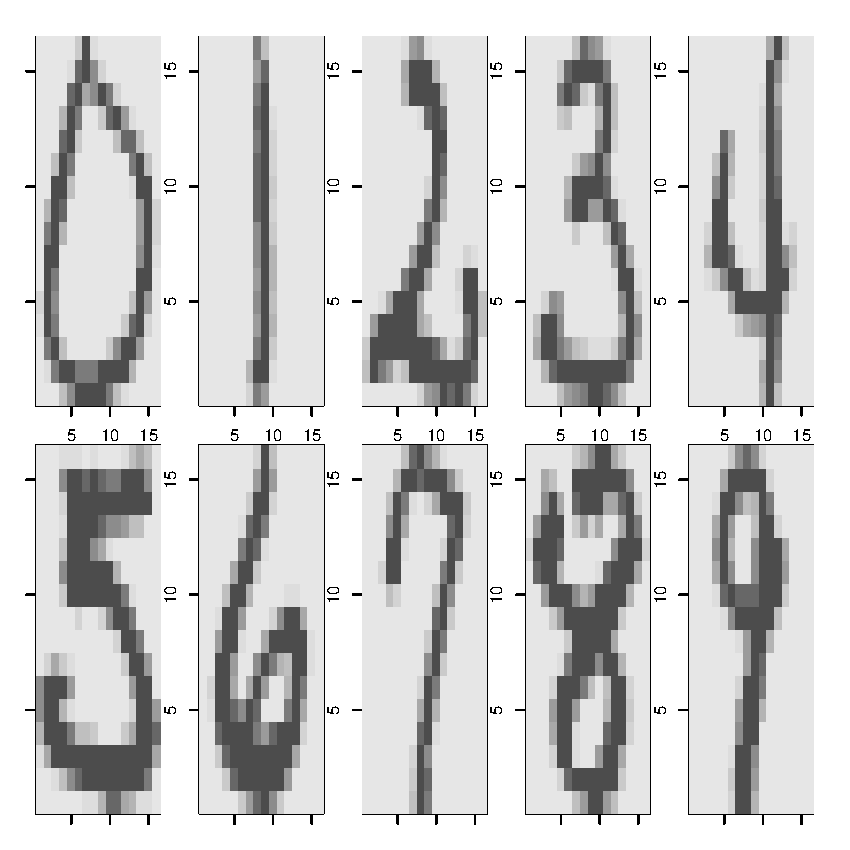
\includegraphics[width=2.0in]
{01Intro/zipdigits.eps}
\end{center}
\caption{ตัวอย่างรูปตัวเลขจากลายมือเขียน}
\label{fig: example ZIP image digits}
\end{figure}
%

%หัวข้อชี้แจง ภาพรวมของการเรียนรู้ของเครื่อง.
%ตลอดตำราเล่มนี้ ผู้เขียนใช้ ฟอนต์เข้ม เช่น $\mathbf{x}$ เพื่อระบุถึงตัวแปรที่เป็นเวกเตอร์ หรือ เมตริกซ์, เพื่อเตือนให้ผู้อ่านนึกภาพตามได้ถูกต้อง เปรียบเทียบกับตัวแปรค่าเดี่ยว เช่น $x$.
%และให้ฟอนต์ \verb|sigmoid| เพื่อแสดงโค้ด ซึ่งต่างจาก $\mathbf{sigmoid}$ ที่แสดงถึงฟังชั่นทางคณิตศาสตร์.

\section{ภาพรวมของการเรียนรู้ของเครื่อง}
\label{sec: ML overview}

\paragraph{ตัวอย่างการรู้จำลายมือแยกตัวเลข.}

รูปที่~\ref{fig: example ZIP image digits} แสดงตัวอย่างรูปภาพที่ต้องการโปรแกรมรู้จำลายมือ เพื่อแยกรูปออกตามตัวเลขที่ภาพแสดง โดยมีรูปภาพของตัวเลขตั้งแต่ $0$ ถึง $9$.
รูปภาพแต่ละรูปเป็น\textit{ภาพขาวดำ} (grayscale) มีขนาด $16 \times 16$ พิกเซล (pixels) 
และ\textit{ค่าของแต่ละพิกเซล}แทนด้วยเลขจำนวนจริง.
ดังนั้น รูปหนึ่งรูปสามารถแทนได้ด้วยตัวแปรเวกเตอร์ของจำนวนจริงขนาด $256$ ($=16 \times 16$) 
หรือคือสามารถกำหนด $\mathbf{x} \in \mathbb{R}^{256}$ แทนรูปหนึ่งรูป.
ในทางปฏิบัติ เราไม่สามารถเขียนโปรแกรมนี้จากกฎตายตัวได้ 
หรือถ้าได้ก็อาจจะได้ผลการทำงานที่แย่มากหรือทำได้ยากมากๆ.

แต่\textit{โปรแกรมรู้จำลายมือแยกตัวเลข}สามารถเขียนขึ้นได้อย่างมีประสิทธิภาพด้วยแนวทางของศาสตร์การเรียนรู้ของเครื่อง.
จุดประสงค์ที่ต้องการคือโปรแกรมที่จะบอกได้ว่า\textit{รูปภาพเป็นรูปภาพของเลขใด} 
หรือกล่าวอีกอย่างคือ การทายฉลาก $y \in \{0, 1, 2, \ldots, 9\}$ ที่เหมาะสม จากรูปภาพ $\mathbf{x}$.

แนวทางของการเรียนรู้ของเครื่องคือจะใช้โมเดลทางคณิตศาสตร์ในการหาค่าเอาท์พุต $y$ จาก อินพุต $\mathbf{x}$ โดย ตัวโมเดลจะถูกควบคุมด้วยพารามิเตอร์ $\bm{\theta}$.
โมเดล $f:\mathbf{x},\bm{\theta} \mapsto y$ อาจเขียนได้เป็น $y = f(\mathbf{x}|\bm{\theta})$ โดย 
$y$ คือ\textit{เอาท์พุต} (หรืออาจจะเรียก\textit{คำตอบ}หรือ\textit{ฉลากของกลุ่ม})
และ $\mathbf{x}$ คือ\textit{อินพุต} หรือเวกเตอร์ค่าของพิกเซล
และ $\bm{\theta}$ คือ\textit{พารามิเตอร์}%
ที่จะสามารถปรับพฤติกรรมการทำงานของโมเดลให้เป็นไปในทางที่ต้องการได้.

โมเดลทางคณิตศาสตร์นี้  
ในทางทฤษฎีแล้ว 
บางโมเดลมีความยืดหยุ่นสูงมาก (เช่น โมเดลโครงข่ายประสาทเทียม) จะสามารถปรับตัวเป็นฟังชั่นอะไรก็ได้ ขึ้นกับการปรับค่าพารามิเตอร์ $\bm{\theta}$.
%
ในการปรับหาค่าพารามิเตอร์ $\bm{\theta}$ ที่เหมาะสม ผู้สร้างโมเดลจะใช้ตัวอย่างของรูปภาพตัวเลข $N$ ภาพ แทนด้วยตัวแปร $\mathbf{X} = [\mathbf{x}_1, \ldots, \mathbf{x}_N]$ พร้อมฉลากเฉลย $N$ ฉลาก แทนด้วยตัวแปรเมตริกซ์ขนาด $1 \times N$ นั่นคือ $\mathbf{T} =[t_1, \ldots, t_N]$.
ฉลากเฉลยนี้อาจได้มาจากการใช้ให้คนดูรูปภาพและระบุฉลากที่ถูกต้องของแต่ละภาพไว้.
ข้อมูล $\mathbf{X}$ และ $\mathbf{T}$ นี้จะถูกเรียกว่า ``ข้อมูลชุดฝึกหัด'' (training dataset).

%นอกจาก รูปภาพตัวเลข $N$ ภาพ: $\mathbf{x}_1, \ldots, \mathbf{x}_N$ แล้ว, ข้อมูลในชุดฝึกหัดนี้ จะมี เฉลย หรือ ตัวอย่างคำตอบ หรือ ฉลากบอกกลุ่มของรูปภาพตัวเลข $t_1, \ldots, t_N$ มาด้วย.
%กล่าวโดยย่อ เราจะมี ตัวอย่างรูป $\mathbf{x}$ และ ตัวอย่างคำตอบ $\mathbf{t}$ เพื่อใช้ในการปรับหาค่าพารามิเตอร์ $\theta$.

อัลกอริทึ่ม\textit{การเรียนรู้ของเครื่อง}จะช่วยหาค่าที่เหมาะสมของพารามิเตอร์ $\bm{\theta}^*$ ออกมา.
ขั้นตอนในการใช้ข้อมูลชุดฝึกหัดเพื่อปรับหาค่าพารามิเตอร์จะเรียกว่า \textit{การฝึกหัด} (training) 
หรือ\textit{การเรียนรู้} (learning).
ผลลัพธ์ที่ได้จาก\textit{การเรียนรู้}คือโมเดลที่พร้อมใช้งาน $f^*(\mathbf{x}) = f(\mathbf{x}|\bm{\theta}^*)$ ที่สามารถใช้ทายค่าฉลากของรูปภาพได้.
นั่นคือ สำหรับรูปภาพ $\mathbf{x}'$ โมเดลจะทายฉลาก $y' = f^*(\mathbf{x}')$.

\paragraph{การประเมินผล.} 
โมเดลที่ดีจะต้องสามารถทายค่าฉลากของรูปภาพใหม่ได้ดี.
รูปภาพใหม่ที่กล่าวถึงนี้ คือรูปภาพที่ไม่ได้ถูกใช้ในขั้นตอนการฝึกโมเดล.
การประเมินผลการทำงานของโมเดลจะใช้ข้อมูลอีกชุด 
โดยที่ข้อมูลชุดนี้จะต้องไม่ได้ถูกใช้ในการฝึกหัด.
ข้อมูลชุดนี้เรียกว่า ``ข้อมูลชุดทดสอบ'' (test dataset).
ความสามารถที่โมเดลทายหรือระบุฉลากของข้อมูลใหม่ได้ดี เรียกว่า \textit{คุณสมบัติความทั่วไป} 
หรือ\textit{คุณสมบัติเจนเนอรอลไลเซชั่น} (Generalization).
เราต้องการโมเดลที่มี\textit{คุณสมบัติความทั่วไป}ที่ดี.
นั่นคือ โมเดลสามารถระบุฉลากได้ถูกต้อง แม้ว่ารูปภาพนั้นจะเป็นรูปใหม่ที่ไม่เคยเห็นมาก่อน.
%
จากตัวอย่างการรู้จำลายมือแยกตัวเลขข้างต้น แม้จะเป็นตัวอย่างง่ายๆ
แต่ภาพรวมและหลักการที่สำคัญหลายๆอย่างที่อภิปรายไปนั้น 
ก็ครอบคลุมแนวทางของการเรียนรู้ของเครื่องโดยทั่วๆไป.

หัวข้อ~\ref{section: Polynomial Curve Fitting} จะอภิปรายฟังชั่นโพลิโนเมียล ที่เป็นโมเดลที่มีรูปแบบทางคณิตศาสตร์ที่ไม่ซับซ้อน %กับ งานการหาค่าถดถอยมิติเดียว, 
ซึ่งน่าจะช่วยให้ผู้อ่านเข้าใจแนวคิดและภาพรวมของการสร้างโมเดลและการปรับหาค่าพารามิเตอร์ได้ดียิ่งขึ้น.
%
บทที่~\ref{chapter: ANN} จะอภิปรายถึงโครงข่ายประสาทเทียม ซึ่งเป็นโมเดลที่มีความซับซ้อนมาก และจัดเป็นหนึ่งในศาสตร์และศิลป์ของวิชาการเรียนรู้ของเครื่อง.
บทที่~\ref{chapter: Applications of ANN} จะสาธิตการประยุกต์ใช้งานโครงข่ายประสาทเทียม
รวมถึงตัวอย่างงานการรู้จำลายมือแยกตัวเลขนี้ เพื่อให้ผู้อ่านได้เห็นภาพโดยสมบูรณ์.

\paragraph{การเตรียมและปรับข้อมูลก่อนและหลัง.} 
ในทางปฏิบัติแล้ว ส่วนใหญ่ อินพุต $\mathbf{x}$ มักจะถูกเตรียมหรือปรับปรุงเบื้องต้นก่อน 
เพื่อเปลี่ยนไปอยู่ในปริภูมิของตัวแปร
(Space of Variables) 
ที่โมเดลจะสามารถทำงานได้ง่ายขึ้น.
ตัวอย่างเช่น อินพุตของโปรแกรมรู้จำลายมือแยกตัวเลข อาจจะถูกปรับให้ ขนาดภาพของตัวเลขแต่ละตัวมีความสูงและความกว้างพอๆกันก่อน 
ซึ่งจะช่วยทำให้สร้างโมเดลเพื่อแยกตัวเลขได้ง่ายขึ้น.
ขั้นตอนในการเตรียมข้อมูลเบื้องต้นนี้ (pre-processing) บางครั้งจะรวมขั้นตอนที่เรียกว่า ``การแยกลักษณะสำคัญ'' (feature extraction) เข้าไปด้วย (ดู~\cite{KatanyukulPonsawat2016a} สำหรับคำอธิบาย และตัวอย่างการแยกลักษณะสำคัญ).
ในบางกรณีการปรับข้อมูลภายหลัง (post-processing) ก็อาจถูกมานำใช้ เพื่อเพิ่มหรือปรับปรุงคุณภาพของเอาท์พุตจากโมเดลได้ เช่น การถอดรหัสแบบหนึ่งไปเค
(1-to-K decoder)
เพื่อปรับเอาต์พุตจากโมเดลจำแนกกลุ่มให้อยู่ในรูปแบบที่ต้องการ (ดูหัวข้อ~\ref{section: multiclass classification} สำหรับรายละเอียด)

\paragraph{ประเภทของการเรียนรู้ของเครื่อง.} 
หากมองจากมุมของประสบการณ์ $E$ ที่คอมพิวเตอร์ใช้ปรับปรุงการทำงาน โปรแกรมรู้จำลายมือแยกตัวเลขต้องการประสบการณ์ ซึ่งคือตัวอย่างอินพุต $\mathbf{X}$ และตัวอย่างเอาท์พุต $\mathbf{T}$.
การเรียนรู้ของเครื่องที่เกี่ยวข้องกับประสบการณ์เช่นนี้ จะเรียกว่า ``การเรียนรู้แบบมีผู้ช่วยสอน'' (Supervised Learning).
\index{Supervised Learning}
\index{การเรียนรู้แบบมีผู้ช่วยสอน}
เมื่อมองจากลักษณะของเอาท์พุต ปัญหาการรู้จำลายมือแยกตัวเลขมีเอาท์พุตเป็นฉลากของกลุ่ม ซึ่งจำนวนกลุ่มมีจำนวนแน่นอน เช่น $10$ กลุ่ม ตั้งแต่ `0' ถึง `9'.
\textit{ปัญหาแบบนี้}จัดเป็นชนิดปัญหาของ\textit{การจำแนกประเภท} (Classification).
แต่หากเอาท์พุตมีลักษณะเป็นเลขจำนวนจริง เช่น การทำนายปริมาณน้ำฝน การทำนายปริมาณแร่ธาตุในดิน การทำนายปริมาณน้ำยางจากต้นยางที่ปลูกในสภาพต่างๆ การทำนายแรงที่เกิดกับใบพัดลักษณะต่างๆของกังหันลม การทำนายมูลค่าการซื้อขายหลักทรัพย์
ปัญหาในลักษณะแบบนี้จะจัดเป็นชนิดปัญหาของ\textit{การหาค่าถดถอย} (Regression).
บทที่~\ref{chapter: Linear Models}~และ~\ref{chapter: ANN} จะอภิปรายถึงการเรียนรู้แบบมีผู้ช่วยสอน ทั้งสองแบบ.

หากประสบการณ์ $E$ ไม่ได้ให้ตัวอย่างเอาท์พุตมาให้ด้วย การเรียนรู้ของเครื่องแบบนี้จะเรียกว่า ``การเรียนรู้แบบไม่มีผู้ช่วยสอน'' (Unsupervised Learning).
\textit{ปัญหาประเภทนี้}มีหลายชนิด เช่น\textit{การจัดกลุ่มข้อมูล} (Clustering) ซึ่งคือการจัดของหรือข้อมูลที่มีลักษณะคล้ายกันให้อยู่กลุ่มเดียวกัน
\textit{การประมาณความหนาแน่นของข้อมูล} (Density Estimation)
\textit{การลดมิติของข้อมูล} (Dimension Reduction) 
หรือแม้แต่\textit{การหาค่าดีที่สุดด้วยวิธีการค้นหาเชิงศึกษาสำนึก} (Optimization with Heuristic Search) 
ซึ่งมีการประยุกต์ใช้อย่างกว้างขวาง และมีรูปแบบวิธีการที่หลากหลาก อาทิ \textit{จีเนติกอัลกอริทึม} (Genetic Algorithm) เป็นต้น
%เราจะศึกษา การเรียนรู้แบบไม่มีผู้ช่วยสอน ใน บทที่~\ref{chapter: others}.

นอกจากนี้ยังมีการเรียนรู้ของเครื่องที่ลักษณะของประสบการณ์ $E$ ต่างจากสองกลุ่มข้างต้น เช่น \textit{การเรียนรู้แบบเสริมกำลัง} (Reinforcement Learning), 
\textit{การเรียนรู้แบบกึ่งมีผู้ช่วยสอน} (Semi-Supervised Learning), 
\textit{การเรียนรู้ของเครื่องที่ใช้ในระบบแนะนำสินค้าอัตโนมัติ} (Recommender Systems) เป็นต้น.
\textit{การเรียนรู้แบบเสริมกำลัง}จะใช้กับปัญหาเชิงลำดับเวลา ที่คอมพิวเตอร์จะเลือกการกระทำที่เหมาะสมกับสถานะในแต่ละคาบเวลา เพื่อที่จะให้ผลรวมของรางวัลในแต่ละคาบเวลามากที่สุด.
ลักษณะของปัญหาที่\textit{การเรียนรู้แบบเสริมกำลัง}ทำงานคือ คอมพิวเตอร์ไม่มีตัวอย่างของการกระทำที่มันควรจะเลือก แต่มันจะค้นหาการกระทำที่เหมาะสมกับสถานะโดยการลองผิดลองถูก เพื่อที่จะเรียนรู้ผลของการกระทำนั้น ในขณะที่ พยายามจะให้ผลรวมของรางวัลมากที่สุดด้วย.
ระบบการเรียนรู้แบบเสริมกำลังที่ดีจะต้องสร้างสมดุล ระหว่างการเลือกการกระทำ เพื่อที่จะได้ผลรวมรางวัลดีที่สุด กับการเลือกการกระทำเพื่อการเรียนรู้.
ประเด็นเรื่องความสมดุลนี้เรียกว่า \textit{ประเด็นของการใช้งานและการเรียนรู้} (issue of exploitation and exploration).
ลักษณะที่เด่นชัดอีกอย่างหนึ่งของการเรียนรู้แบบเสริมกำลัง คือการที่ระบบมีปฏิสัมพันธ์สิ่งแวดล้อม ผลของการกระทำที่ระบบเลือกมีผลต่อสิ่งที่ระบบจะเรียนรู้ (ดู~\cite{KatanyukulEtAl2011a} หรือ \cite{SuttonBarto1998a} สำหรับรายละเอียด)
%เราจะศึกษาการเรียนรู้แบบเสริมกำลัง ในบทที่~\ref{chapter: others}.

บทที่~\ref{chapter: Optimization}
อภิปรายศาสตร์การหาค่าดีที่สุดเบื้องต้น 
ซึ่งศาสตร์การหาค่าดีที่สุดเป็นพื้นฐานที่สำคัญ 
สำหรับอธิบายกลไกการทำงานของวิชาการเรียนรู้เครื่อง.
%
บทที่~\ref{chapter: background} อภิปรายตัวอย่างง่ายๆที่จะช่วยให้เห็นภาพของการเรียนรู้ของเครื่อง การประเมินผล และการเลือกโมเดล เพื่อความเข้าใจก่อนที่จะศึกษาโมเดลที่ซับซ้อนขึ้น
%: วิธีการหาค่าดีที่สุด, ตัวอย่างการหาค่าถดถอยมิติเดียวด้วยฟังชั่นพหุนาม, ทฤษฏีความน่าจะเป็น, การแบ่งกลุ่มด้วยโลจิสติกส์ถดถอย, และ การเลือกโมเดล.
%
บทที่~\ref{chapter: Linear Models} อภิปรายโมเดลเชิงเส้น ซึ่งมีรูปแบบคณิตศาสตร์ที่เข้าใจง่ายไม่ซับซ้อน.
บทที่~\ref{chapter: ANN}~และ~\ref{chapter: Applications of ANN} อภิปรายโมเดลโครงข่ายประสาทเทียม และการนำไปประยุกต์ใช้งาน.
บทที่~\ref{chapter: Suggestions for ANN} อภิปรายเทคนิคและแนวทางในการนำโครงข่ายประสาทเทียมไปใช้ในทางปฏิบัติ.
%บทที่~\ref{chapter: ANN deep learning} อภิปรายทิศทางการพัฒนาในปัจจุบันของโครงข่ายประสาทเทียม.


%\begin{minipage}{5.5in}
%{\small
%\begin{shaded}
%การหาค่าดีที่สุดด้วยการค้นหาปฏิสัมพันธ์ (อังกฤษ Reactive Search and Intelligent Optimization, คำย่อ RSO)

%โครงข่ายเบย์เซียน (อังกฤษ Bayesian Network)

%\end{shaded}
%}
%\end{minipage}

%\begin{minipage}{5.5in}
{\small
\begin{shaded}
\paragraph{\small เกร็ดความรู้ สติปัญญาของลิง}
\index{สติปัญญา}\index{Intelligence}
ปี ค.ศ. 2008 สถานีโทรทัศน์พีบีเอสของสหรัฐอเมริกาออกอากาศรายการ\textit{โนวา} เกี่ยวกับสติปัญญาของลิงไม่มีหาง เรื่อง ``Ape Genius''
รายการนำเสนองานศึกษาสติปัญญาของลิงชิมแปนซีและลิงโบโนโบหลายๆงาน (ลิงชิมแปนซีและลิงโบโนโบ มีพันธุ์กรรมต่างจากมนุษย์แค่ประมาณ $1.2\%$
(มนุษย์แต่ละคนมีพันธุ์กรรมแตกต่างกันประมาณ $0.1\%$
จาก \verb|http://humanorigins.si.edu/evidence/genetics| สืบค้น 12 สิงหาคม 2559)
รายการดำเนินการ โดยเป้าหมายคือ เพื่อหาคำตอบว่า ลักษณะของสติปัญญาแง่มุมใดที่ต่างกัน และทำให้ชิมแปนซีและโบโนโบไม่สามารถพัฒนาขึ้นมาสร้างอารยธรรม เช่นเดียวกับที่มนุษย์ทำได้.
%\begin{itemize}
%\item 

ความสามารถในการสร้างและใช้เครื่องมือ.
มีหลักฐานชัดเจนว่า ลิงชิมแปนซีมีการสร้างและใช้เครื่องมือ เช่น การสังเกตุของ\textit{เจน กูดดอล} ที่พบลิงชิมแปนซีในแทนซาเนียใช้กิ่งไม้ในการล่อมดมากิน
และ\textit{จิล พริตซ์}ที่พบลิงชิมแปนซีในป่า\textit{โฟกอลี}ในประเทศเซเนกัล ที่สร้างหอกจากกิ่งไม้และใช้เป็นเครื่องมือในการล่าหาอาหาร
%อีกทั้งลิงอีกหลายๆตัวในฝูงก็สามารถสร้างและใช้เครื่องมือในแบบเดียวกันได้
%\item 

ความสามารถในการทำงานร่วมกัน.
มีหลักฐานหลายอย่างแสดงให้เห็นพฤติกรรมในลักษณะการออกล่าร่วมกันของลิงชิมแปนซี
และมีการทดลองของสถาบันวิจัยลิงใหญ่ไม่มีหาง (Great Ape Research Institute) ของญี่ปุ่น
ที่พบว่าลิงชิมแปนซีมีความสามารถในการทำงานร่วมกัน มีความสามารถในการขอความช่วยเหลือ และก็สามารถให้ความช่วยเหลือมนุษย์ได้เวลาที่ถูกร้องขอ
%\item 

ความสามารถในการแก้ปัญหา.
การศึกษาหนึ่งทดลอง โดยใส่เมล็ดถั่วไว้ในหลอดยาวที่ลิงไม่สามารถจะล้วงเข้าไปหยิบได้
และตัวหลอดก็ยึดติดกับกรงแน่นจนลิงไม่สามารถขยับได้.
ลิงใช้เวลาพักหนึ่ง ก่อนจะพบวิธีแก้ปัญหา.
มันไปที่บ่อน้ำในกรง อมน้ำแล้วมาพ่นใส่หลอด แล้วอาหารก็ลอยขึ้นบนน้ำ 
มันเติมน้ำเข้าไปจนอาหารลอยอยู่ในระดับที่เอื้อมถึงได้
สิ่งนี้แสดงถึงความสามารถในการแก้ปัญหาของลิง.
%\item 

ความสามารถในการเลียนแบบ.
ทีมของนักจิตวิทยา\textit{แอนดรู วิทเทน}ต้องการทดสอบความสามารถในการเลียนแบบของลิง.
ทีมสร้างเครื่องกลไกที่ลิงจะต้องทำ $2$ ขั้นตอนได้แก่ หมุนจานให้พอดีช่องและโยกคันโยก เพื่อจะได้กินอาหาร
และนำเครื่องไปทดสอบกับตัวลิง.
ลิงไม่สามารถจะหาวิธีทำนี้ได้เอง.
แต่ทีมงานค่อยๆสอนลิงขึ้นมาตัวหนึ่ง
จากนั้นลองให้ลิงตัวอื่นดูลิงตัวนี้ทำงาน
แล้วสังเกตุว่าลิงตัวอื่นๆก็สามารถเลียนแบบ เพื่อทำงานสองขั้นตอนนี้ได้อย่างง่ายดาย.

ความสามารถทางตัวเลข.
\textit{เททซูโร มัตซูซาวา}แห่งมหาวิทยาลัยเกียวโต นำเสนอผลการทดสอบลิงชิมแปนซีชื่อ\textit{ไอ} ที่แสดงความสามารถทางตัวเลข ในการเข้าใจความหมายของตัวเลขอารบิก และยังสามารถรู้ลำดับของตัวเลขได้

ความสามารถทางภาษาและการสื่อสาร.
ลิงโบโนโบชื่อ\textit{คานซี} เรียนรู้ภาษาอังกฤษได้เอง โดยไม่ได้ถูกสอนโดยตรง
และ\textit{ซู ซาเวจ-รัมบาว}แสดงให้เห็นว่า\textit{คานซี}เข้าใจภาษาอังกฤษและสามารถทำตามคำสั่งได้อย่างถูกต้อง

\paragraph{\small ความสามารถที่ลิงไม่มี} 
ความสามารถที่กล่าวมาข้างต้น เป็นความสามารถที่พบหลักฐานในลิงชิมแปนซีหรือโบโนโบ.
แต่ความสามารถที่ลิงชิมแปนซีหรือโบโนโบไม่มี
และเป็นปัจจัยสำคัญที่ทำให้ลิงไม่สามารถพัฒนาอารยธรรมขึ้นมาได้
เชื่อว่าคือ\textit{ความสามารถด้านอารมณ์}.
ลิงชิมแปนซีมีปัญหาที่เห็นได้ชัดเจน คือปัญหาด้านอารมณ์ ทั้งการแก่งแย่งชิงดีกัน ความรุนแรง และที่สำคัญคือ การควบคุมอารมณ์ตัวเอง.

ความสามารถในการควบคุมตัวเอง.
การทดลองของ\textit{แซลลี่ บอยเซน}มหาวิทยาลัยรัฐโอไอโอ
แสดงให้เห็นโดยให้ลิงเลือกจานอาหารระหว่างจาน $2$ จานที่มีขนมอยู่ไม่เท่ากัน
แต่จานที่ลิงเอื้อมมือไปหา จะเป็นจานที่จะไปให้กับลิงอีกตัว.
ถ้าเป็นขนมที่อยู่บนจาน ลิงไม่สามารถจะอดใจและเอื้อมไปที่จานที่น้อยกว่าได้
มันจะเอื้อมไปที่จานที่มันเห็นอาหารมากกว่าตลอด.
แต่พอ\textit{แซลลี่ บอยเซน}เปลี่ยนจากการที่เอาขนมวางไว้ในจานให้เห็น
กลับใช้ตัวเลขซึ่งลิงเข้าใจความหมาย วางไว้แทน.
ลิงสามารถเรียนรู้ที่จะเอื้อมไปที่จานที่ตัวเลขน้อยกว่าได้.
การทดลองนี้แสดงให้เห็นว่า ลิงชิมแปนซีมีปัญหาในการควบคุมอารมณ์ของตัวมันเอง.
เวลาที่มันเห็นอาหารอยู่ มันไม่สามารถควบคุมตัวเพื่อเลือก\textit{ทางเลือกที่ดีกว่า}ได้
แต่พอตัดแรงกระตุ้นทางอารมณ์ออก (ใช้ตัวเลขวางแทนอาหารจริง) มันสามารถเลือก\textit{ทางเลือกที่ดีกว่า}ได้.

นอกจากการขาดความสามารถในการควบคุมตนเองแล้ว
ปัจจัยสำคัญอีกสองอย่างที่รายการสรุปว่า เป็นอุปสรรคที่ทำให้สติปัญญาของลิงไม่อาจสะสม สร้างเสริมไปสู่การพัฒนาในระดับเดียวกับมนุษย์ได้ ก็คือ
ความสามารถในการเรียนรู้โดยรับการถ่ายทอดจากคนอื่น (หรือลิงตัวอื่น)
และความสามารถในการสอน.
แม้เด็กอาจไม่ได้แสดงความสามารถในการแก้ปัญหาได้ดีเท่ากับลิงชิมแปนซี
แต่เด็กๆแสดงความสามารถที่สามารถเรียนรู้จากสิ่งที่ถูกสอนได้ดีกว่า
สุนัขเองก็ยังมีความสามารถในการเรียนจากการสอนของมนุษย์ได้ดีกว่าลิง.

นอกจากความสามารถในการเรียนจากการถ่ายทอด
ความเต็มใจที่จะถ่ายทอด หรือความเต็มใจที่จะสอน ก็เป็นส่วนประกอบสำคัญที่ทำให้การถ่ายทอดความรู้เกิดขึ้นได้
และลิงชิมแปนซีไม่มีทั้งสององค์ประกอบนี้.
อารยธรรมของมนุษย์สร้างโดยการส่งผ่านความรู้และปัญญาจากรุ่นสู่รุ่น.
แม้ลิงสามารถเรียนรู้จากลิงตัวอื่นได้โดยการเลียนแบบ
แต่การเรียนรู้โดยการเลียนแบบนั้นมักจะช้าและตื้นเขิน.
บางครั้งยังอาจมีการสูญหายไป จากการเปลี่ยนรุ่นของลิงอีกด้วย.
ลิงรุ่นเก่าตายไป ลิงรุ่นใหม่อาจไม่ได้เรียนรู้สิ่งที่ลิงรุ่นเก่ารู้แล้ว
หลายๆอย่างที่ลิงรุ่นเก่ารู้แล้ว เช่นวิธีการใช้เครื่องมือ อาจหายไปจากลิงรุ่นใหม่
และอาจใช้เวลาอีกนานกว่าที่ลิงรุ่นใหม่จะพบวิธีใช้เครื่องมืออีกครั้ง.

การควบคุมตัวเอง การเรียนรู้จากการถ่ายทอด และความเต็มใจที่จะสอน เป็นคุณสมบัติที่แยกมนุษย์ออกจากลิง 
และเป็นพื้นฐานอารยธรรมของมนุษย์.
%สิ่งที่เราเรียนรู้จากสติปัญญาของลิง หวังว่าจะช่วยบอกวิธีที่เราจะใช้สติปัญญาของเรา
\end{shaded}
}
%\end{minipage}


\section{กิจกรรมเชิงปฏิบัติ}
การเรียนรู้ของเครื่องเป็นศาสตร์และศิลป์ของการนำทฤษฏีไปประยุกต์กับการปฏิบัติ 
และวิธีที่ดีที่สุดในการเรียนรู้\textit{ศาสตร์การเรียนรู้ของเครื่อง} ก็คือ การลองลงมือทำ.
แม้จะมีเครื่องมือที่ใช้ได้มากมาย ไม่ว่าจะเป็น แมทแลป ไพธอน อาร์โปรเจค
%Matlab, Python, R project, 
หรือว่าภาษาโปรแกรมทั่วๆไป เช่น 
ซี ซีพลัสพลัส หรือจาวา เป็นต้น
%C, C++, Java เป็นต้น.
%จากตัวเลือกมากมาย 
หนังสือเล่มนี้เลือก\textit{อาร์โปรเจค} (R Project) เป็นเครื่องมือสำหรับเสริมเนื้อหาของหนังสือนี้
บนพื้นฐานของความสามารถในการคำนวณที่ดี และประสิทธิภาพในการประมวลผลข้อมูลขนาดใหญ่  รวมถึงการที่\textit{อาร์โปรเจค}ติดตั้งง่าย และมีเสถียรภาพพอสมควร. 
นอกจากนั้น อาร์โปรเจคยังเป็น\textit{โปรแกรมรหัสเปิด}ที่สนันสนุนหลากหลายระบบปฏิบัติการ และมีฐานผู้ใช้จำนวนมาก.

ผู้อ่านสามารถดาวน์โหลดและติดตั้งโปรแกรมอาร์โปรเจคได้ตามคำแนะนำจากเวปไซต์ \verb|https://www.r-project.org/|
หลังจากติดตั้งโปรแกรมเรียบร้อยแล้ว 
หัวข้อ~\ref{sec: basic R examples} แสดงตัวอย่างการใช้\textit{โปรแกรมอาร์}เบื้องต้น พร้อมคำอธิบายสั้นๆ.

\subsection{การใช้อาร์โปรเจคเบื้องต้น}
\label{sec: basic R examples}
ตัวอย่างต่อไปนี้ (แสดงข้างล่างในรูปแบบสองคอลัมน์) แสดงการบวก ลบ คูณ หาร หารเอาเศษ (modulus) ยกกำลัง เปรียบเทียบมากกว่า เปรียบเทียบมากกว่าหรือเท่ากับ เปรียบเทียบเท่ากับ เปรียบเทียบไม่เท่ากับ เปรียบเทียบน้อยกว่า และการใช้วงเล็บ.
บรรทัดที่นำหน้าด้วยเครื่องหมาย \verb|>| เป็นคำสั่งที่ผู้ใช้ใส่เข้าไป ส่วนบรรทัดที่นำหน้าด้วย \verb|[1]| คือคำตอบที่ได้จากอาร์โปรเจค.

\begin{multicols}{2}
\begin{verbatim}
> 5 + 4
[1] 9
> 5 - 4
[1] 1
> 5 * 4
[1] 20
> 5 / 4
[1] 1.25
> 5 %% 4
[1] 1
> 2^5
[1] 32
> 5 > 3
[1] TRUE
> 5 >= 3
[1] TRUE
> 5 == 3
[1] FALSE
> 5 != 3
[1] TRUE
> 5 < 3
[1] FALSE
> (5 < 3) == TRUE
[1] FALSE
\end{verbatim}
\end{multicols}

ตัวอย่างข้างล่างในรูปแบบสองคอลัมน์ แสดง การใช้ฟังชั่นสำเร็จรูป ได้แก่ \verb|pi| สำหรับค่า $\pi$, 
ค่าฟังชั่นไซน์, 
ค่า $e^1$, 
ค่าล๊อกการิทั่มของ $0.1$, $0$, $10$ และ $e^5$, 
การปัดเศษเป็นจำนวนเต็ม และเป็นทศนิยม $1$ ตำแหน่ง 
และการดูเวลาของระบบ.
สังเกตุ มหัพภาพ (เครื่องหมายจุด) สำหรับอาร์โปรเจค เป็นแค่\textit{ตัวอักขระ}ธรรมดาเหมือน \verb|a|, \verb|b|, \verb|c| เป็นต้น ไม่ได้มีความหมายพิเศษ.
สำหรับอาร์โปรเจค \textit{มหัพภาพ}ไม่ใช่เครื่องหมายบ่งชี้แอททรีบิวต์ (attribute) หรือเมธอด (method) ของการเขียน\textit{โปรแกรมเชิงวัตถุ}

\begin{multicols}{2}
\begin{verbatim}
> pi
[1] 3.141593
> sin(pi/2)
[1] 1
> exp(1)
[1] 2.718282
> log(0.1)
[1] -2.302585
> log(0)
[1] -Inf
> log(10)
[1] 2.302585
> log(exp(5))
[1] 5
> round(545.32)
[1] 545
> round(545.32,1)
[1] 545.3
> Sys.time()
[1] "2013-09-05 10:59:32 ICT"
\end{verbatim}
\end{multicols}

ตัวอย่างข้างล่างในรูปแบบสองคอลัมน์ แสดงการให้ค่าตัวแปร การเรียกตัวแปร การเรียกตัวแปรที่ยังไม่ได้ประกาศ.
สังเกตุ (1) ตัวใหญ่ตัวเล็กไม่เหมือนกัน
(2) เทอม \texttt{my.x} เป็นแค่ชื่อตัวแปร เช่นเดียวกับ \textit{ภาษาซี}ที่มักใช้\textit{ขีดล่าง}แยกคำ เช่น \verb|my_x| 
ย้ำอีกครั้งมหัพภาค(เครื่องหมายจุด)ไม่ได้มีความหมายพิเศษสำหรับอาร์โปรเจค
(3) อาร์โปรเจคใช้ \verb|=| หรือ \verb|<-| เป็น\textit{ตัวปฏิบัติการให้ค่า} (assignment operator).

\begin{multicols}{2}
\begin{verbatim}
> x <- 5
> x
[1] 5
> X
Error: object 'X' not found
> X <- 8
> X
[1] 8
> x
[1] 5
> x <- X + 8
> x
[1] 16
> x = 4
> x
[1] 4
> my.x <- 23
> my.x
[1] 23
\end{verbatim}
\end{multicols}

ตัวอย่างการนิยามฟังชั่น. 
สังเกตุ 
(1) ถ้าภายในตัวฟังชั่นไม่มีการเรียก \verb|return| อาร์โปรเจคจะเอาค่าที่ได้จากคำสั่งบรรทัดสุดท้ายตัวฟังชั่นออกมาตอบ (ดู \verb|f0| เทียบกับ \verb|my.f0|)
(2) ถ้าเรียกชื่อฟังชั่นโดยไม่ใส่วงเล็บตามหลัง อาร์โปรเจคจะพิมพ์โค้ดของฟังชั่นออกมา (ดู \verb|f2|)
(3) อาร์โปรเจคอนุญาติให้สามารถใส่อาร์กูเมนต์ตามลำดับ หรือใส่ชื่อเข้าไปได้ (ดูการเรียกใช้ \verb|f2|).

%\begin{multicols}{2}
\begin{verbatim}
> f0 <- function(){ 1; 5; 9; }
> f0()
[1] 9
> f0 <- function(){ 1; 5; 9; 3}
> f0()
[1] 3
> my.f0 <- function(){ 1; return(5); 9; 3}
> my.f0()
[1] 5
> f2 <- function(a, b){ a - b }
> f2
function(a, b){ a - b }
> f2(5, 9)
[1] -4
> f2(a=5, b=9)
[1] -4
> f2(b=5, a=9)
[1] 4
\end{verbatim}
%\end{multicols}

ตัวอย่างการดูคำอธิบายและการหาฟังชั่นที่ต้องการ.
สังเกตุและเปรียบเทียบผลจากการรันสองคำสั่งข้างล่าง.
\begin{verbatim}
> help(seq)
> ??seq
\end{verbatim}

\subsection{ตัวแปรหลายค่าและเมตริกซ์}

ตัวอย่างการกำหนดค่าให้กับ\textit{ตัวแปรหลายค่า}และ\textit{ตัวแปรเมตริกซ์}.
สังเกตุ (1) วิธีการสร้างตัวแปรหลายค่าและผลที่ได้
(2) การสร้างเมตริกซ์ของอาร์โปรเจค จะเรียกตัวเลขตามคอลัมน์โดยดีฟอล์ต ถ้าอยากให้เรียกตามแถวต้องระบุ \verb|byrow=T| หรือ \verb|byrow=TRUE|.
\begin{verbatim}
> seq(0, 1, len=5)
[1] 0.00 0.25 0.50 0.75 1.00
> seq(0, 1, by=0.2)
[1] 0.0 0.2 0.4 0.6 0.8 1.0
> x <- seq(-1, 1, len=5)
> x
[1] -1.0 -0.5  0.0  0.5  1.0
> 1:5
[1] 1 2 3 4 5
> seq(1, 5)
[1] 1 2 3 4 5
> x <- 1:3
> x
[1] 1 2 3
> y <- seq(0, 0, len=3)
> y
[1] 0 0 0
> m1 <- matrix(0, 2, 3)
> m1
     [,1] [,2] [,3]
[1,]    0    0    0
[2,]    0    0    0
> m2 <- matrix(8, 2, 3)
> m2
     [,1] [,2] [,3]
[1,]    8    8    8
[2,]    8    8    8
> m1 <- matrix(1:6, 2, 3)
> m1
     [,1] [,2] [,3]
[1,]    1    3    5
[2,]    2    4    6
> m1 <- matrix(c(24, 6, 2475, 4, 7, 1776), 2, 3)
> m1
     [,1] [,2] [,3]
[1,]   24 2475    7
[2,]    6    4 1776
> m1 <- matrix(c(24, 6, 2475, 4, 7, 1776), 2, 3, byrow=T)
> m1
     [,1] [,2] [,3]
[1,]   24    6 2475
[2,]    4    7 1776
\end{verbatim}

ตัวอย่างการอ้างค่าตัวแปรหลายค่าและเมตริกซ์.
สังเกตุ (1) การใช้ฟังชั่น \verb|dim| ในการดูขนาดของเมตริกซ์
(2) ถ้าแยกส่วนของเมตริกซ์ออกมา แล้วส่วนที่แยกออกมาเป็นแต่แถวเดียวหรือหลักเดียว อาร์โปรเจคจะเปลี่ยนเมตริกซ์เป็นตัวแปรหลายค่า (ดูผล \verb|y[-2,]| เปรียบเทียบกับ
\verb|y[-2,,drop=F]|).
ถ้าผู้ใช้อยากจะให้ผลลัพธ์คงชนิดเป็นเมตริกซ์ ต้องระบุอาร์กูเมนต์ \verb|drop=F| หรือ \verb|drop=FALSE| เข้าไป.

\begin{verbatim}
> x <- seq(1,10, by=2)
> x
[1] 1 3 5 7 9
> x[4]
[1] 7
> x[-4]
[1] 1 3 5 9
> x[2:4]
[1] 3 5 7
> x[-2:-4]
[1] 1 9
> x[c(1,4)]
[1] 1 7
> y <- matrix(seq(1,10, len=6), 2,3, byrow=T)
> y
     [,1] [,2] [,3]
[1,]  1.0  2.8  4.6
[2,]  6.4  8.2 10.0
> y[2,3]
[1] 10
> y[2,]
[1]  6.4  8.2 10.0
> y[,2]
[1] 2.8 8.2
> y[,2:3]
     [,1] [,2]
[1,]  2.8  4.6
[2,]  8.2 10.0
> y[,c(1,3)]
     [,1] [,2]
[1,]  1.0  4.6
[2,]  6.4 10.0
> dim(y)
[1] 2 3
> y[,-1]
     [,1] [,2]
[1,]  2.8  4.6
[2,]  8.2 10.0
> dim(y[,-1])
[1] 2 2
> y[-2,]
[1] 1.0 2.8 4.6
> dim(y[-2,])
NULL
> length(y[-2,])
[1] 3
> class(y)
[1] "matrix"
> class(y[-2,])
[1] "numeric"
> y[-2,,drop=F]
     [,1] [,2] [,3]
[1,]    1  2.8  4.6
> class(y[-2,,drop=F])
[1] "matrix"
> y[,-1:-2]
[1]  4.6 10.0
> class(y[,-1:-2])
[1] "numeric"
\end{verbatim}

ตัวอย่างการบวกเมตริกซ์ การคูณสเกล่าร์กับเมตริกซ์ การลบเมตริกซ์
\textit{การคูณแบบตัวต่อตัว} (Element-Wise Multiplication) 
การทำเมตริกซ์ทรานสโพต์ (Matrix Transpost)
การคูณเมตริกซ์
การทำเมตริกซ์อินเวอร์ส (Matrix Inverse)
และการสร้าง\textit{เมตริกซ์เส้นทแยง} (Diagonal Matrix).

\begin{verbatim}
> y
     [,1] [,2] [,3]
[1,]  1.0  2.8  4.6
[2,]  6.4  8.2 10.0
> y + y
     [,1] [,2] [,3]
[1,]  2.0  5.6  9.2
[2,] 12.8 16.4 20.0
> 2*y
     [,1] [,2] [,3]
[1,]  2.0  5.6  9.2
[2,] 12.8 16.4 20.0
> 2*y - y
     [,1] [,2] [,3]
[1,]  1.0  2.8  4.6
[2,]  6.4  8.2 10.0
> y * y
      [,1]  [,2]   [,3]
[1,]  1.00  7.84  21.16
[2,] 40.96 67.24 100.00
> y %*% y
Error in y %*% y : non-conformable arguments
> t(y)
     [,1] [,2]
[1,]  1.0  6.4
[2,]  2.8  8.2
[3,]  4.6 10.0
> y %*% t(y)
      [,1]   [,2]
[1,] 30.00  75.36
[2,] 75.36 208.20
> t(y) %*% y
      [,1]  [,2]   [,3]
[1,] 41.96 55.28  68.60
[2,] 55.28 75.08  94.88
[3,] 68.60 94.88 121.16
> x <- matrix(seq(1,9, len=4), 2, 2)
> x
         [,1]     [,2]
[1,] 1.000000 6.333333
[2,] 3.666667 9.000000
> solve(x)
           [,1]       [,2]
[1,] -0.6328125  0.4453125
[2,]  0.2578125 -0.0703125
> solve(x) %*% x
              [,1]          [,2]
[1,]  1.000000e+00 -3.885781e-16
[2,] -3.585999e-17  1.000000e+00
> z <- diag(4)
> z
     [,1] [,2] [,3] [,4]
[1,]    1    0    0    0
[2,]    0    1    0    0
[3,]    0    0    1    0
[4,]    0    0    0    1
\end{verbatim}

\subsection{การเขียนโปรแกรมด้วยอาร์สคริปต์}
ตัวอย่างที่ผ่านมาเป็นการใช้อาร์โปรเจคในลักษณะของรันคำสั่งเดี่ยวๆ
การใช้งานอาร์โปรเจคสามารถที่จะรวบรวมคำสั่งเดี่ยวๆเพื่อเขียนเป็นโปรแกรมได้
เช่น ตัวอย่างการใช้คำสั่ง \verb|if| ในการควบคุมลำดับของโปรแกรม.
\begin{verbatim}
> a <- 3
> 
> if(a > 2){
+ 
+    cat('a is greater than 2.\n')
+ }
a is greater than 2.
> a <- 1
> 
> if(a > 2){
+ 
+    cat('a is greater than 2.\n')
+ }
\end{verbatim}

ตัวอย่างการใช้ \verb|if ... else|.
\begin{verbatim}
> a <- 1
> 
> if(a > 2){
+ 
+    cat('a is greater than 2.\n')
+ }else{
+    cat('a is not greater than 2.\n')
+ }
a is not greater than 2.
\end{verbatim}

ตัวอย่างการใช้ \verb|for|.
สังเกตุการใช้คำสั่ง \texttt{paste} เพื่อรวมข้อความกับค่าตัวแปร.

\begin{verbatim}
> a <- 0
> 
> for(i in 1:4){
+ 
+    cat(paste('a = ', a, '\n'))
+    a <- a + 1
+ }
a =  0 
a =  1 
a =  2 
a =  3 
\end{verbatim}

ตัวอย่างการใช้คำสั่ง \verb|for| ร่วมกับ \verb|break|. 
สังเกตุการทำงาน และ ลองรัน \verb|??control| เพื่อศึกษาคำสั่งอื่นๆที่ใช้ควบคุมลำดับของโปรแกรม เช่น \verb|while| และ \verb|repeat| เป็นต้น.

\begin{verbatim}
> a <- 0
> 
> for(i in 1:4){
+ 
+    cat(paste('a = ', a))
+    a <- a + 1
+    if(a > 2) break;
+    cat('; done updating a\n')
+ }
a =  0; done updating a
a =  1; done updating a
a =  2
\end{verbatim}

\paragraph{การโหลดซอร์สโค้ดและเรียกไลบรารี}
ผู้ใช้สามารถเขียนโปรแกรมเป็นสคริปต์ไว้แล้วเรียกใช้ภายหลังได้ %อาร์โปรเจครันมันทีเดียวได้
เช่น ผู้ใช้อาจเขียนโปรแกรมข้างล่างนี้แล้วบันทึก เป็นไฟล์ชื่อ \verb|nparks.r|.

\begin{verbatim}
list.parks <- function(i=NULL){
   parks.to.see <- c('Khao yai', 'Keang Krachan', 'Pha tam')

   N <- length(parks.to.see)

   if(is.null(i)){
      i <- 1:N
   }
   for(p in i){
      cat(paste('park: ', parks.to.see[p], '\n'))
   }

}

list.parks()
\end{verbatim}

หลังจากบันทึกไฟล์ข้างต้นแล้ว ที่\textit{หน้าต่างส่วนรับคำสั่ง} (Command Session) ของอาร์โปรเจค 
ให้ทดลองเรียก \verb|source('nparks.r')|. 
สังเกตุผลและวิธีการรันสคริปต์ของอาร์โปรเจค.
ถ้าอาร์โปรเจคหาไฟล์ไม่เจอ ให้ลองตรวจสอบดูว่า\textit{ไฟล์ที่บันทึก}ได้บันทึกอยู่ที่ไดเรกทอรีเดียวกับไดเรกทอรีที่อาร์โปรเจคทำงานอยู่หรือไม่
% \verb|working directory| ของอาร์โปรเจค. 
ให้ลองศึกษาวิธีการใช้คำสั่ง \verb|getwd| คำสั่ง \verb|setwd| รวมถึงวิธีการใส่เส้นทางที่อยู่ (path) %
% path 
หน้าชื่อไฟล์สำหรับการใช้คำสั่ง \verb|source| เพื่อระบุที่อยู่ของไฟล์.

อาร์โปรเจคมีไลบรารีให้เลือกใช้มากมาย.
ไลบรารีของอาร์โปรเจค มีลักษณะเดียวกับ library ในภาษาซี, package ในจาวา, หรือ toolbox ในแมทแลป. การเรียกใช้ไลบรารีก็เพียงแค่เรียก \verb|library(...)| โดยใส่ชื่อไลบรารีที่ต้องการเข้าไป 
เช่น
ลอง \verb|library(MASS)| และศึกษาการใช้คำสั่ง \verb|mvrnorm| ซึ่งเป็นคำสั่งในไลบรารี \verb|MASS|.
ถ้าโหลดไลบรารีไม่ได้ อาจเป็นเพราะเรายังไม่ได้ติดตั้ง ไลบรารี \verb|MASS|.
ดูวิธีการติดตั้งไลบรารีโดยเรียก \verb|??install.packages|.

\paragraph{การบันทึกข้อมูลและนำเข้าข้อมูล}
ตัวอย่างข้างล่างแสดงการบันทึกค่าตัวแปร \verb|x|.
สังเกตุการทำงานและศึกษาคำสั่ง \verb|runif|.
\begin{verbatim}
> x <- runif(3)
> x
[1] 0.3249652 0.7399444 0.9919758
> save(x, file='savX.RData')
\end{verbatim}
ตอนนี้หากดูในไดเรกทอรีที่ทำงานอยู่ จะพบว่ามีไฟล์ \texttt{savX.RData} ปรากฏขึ้นมา.
การนำเข้าค่าจากไฟล์ที่บันทึกไว้ ก็เพียงเรียก
\begin{verbatim}
load('savX.RData')
\end{verbatim}

\paragraph{การวาดกราฟ}
โปรแกรมข้างล่างนี้แสดงการวาดกราฟดังแสดงในรูปที่~\ref{fig: R plot}.
\begin{verbatim}
> x <- seq(0, 2*pi, len=30)
> plot(x, sin(x))
\end{verbatim}

หากผู้ใช้ต้องการวาดกราฟเป็นเส้นสามารถกำหนดได้โดย การระบุ \verb|type='l'| เข้าไป เป็น \verb|plot(x, sin(x), type='l')|.
ลองศึกษาการทำงานของ \verb|plot| (โดยลอง \verb|help(plot)|).

%
\begin{figure}
\begin{center}
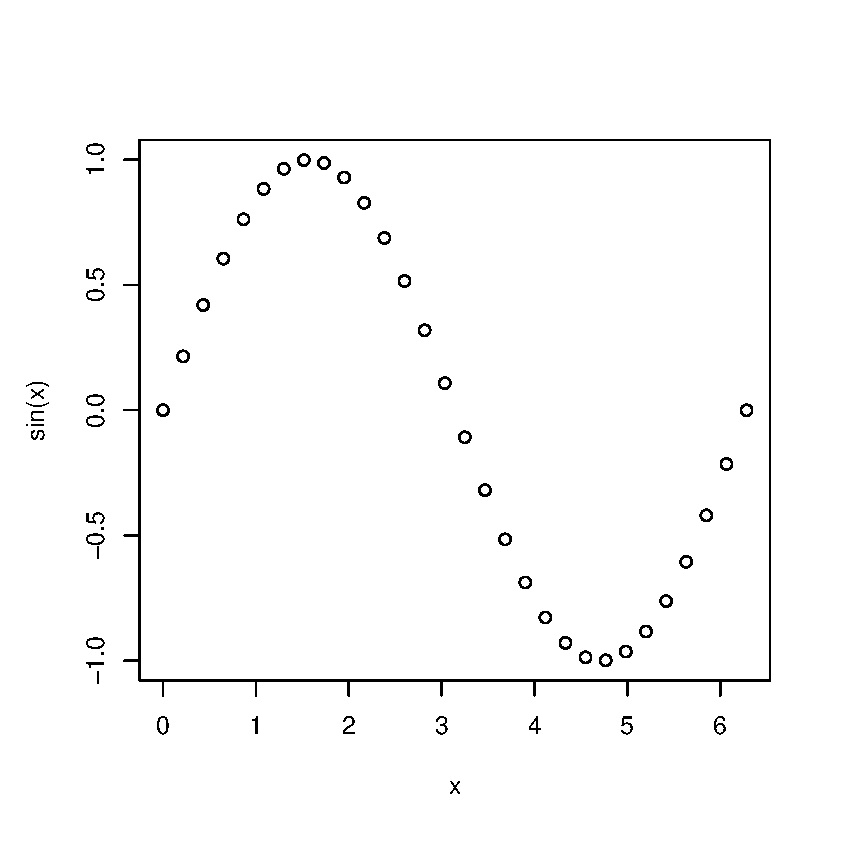
\includegraphics[width=3.0in]
{01Intro/Rplot01.eps}
\end{center}
\caption{ตัวอย่างจากคำสั่ง \texttt{plot}}
\label{fig: R plot}
\end{figure}
%

\section{แบบฝึกหัด}

\paragraph{1.} จงสืบค้นจากอินเตอร์เนตเพื่อหาตัวอย่างการประยุกต์ใช้การเรียนรู้ของเครื่องอย่างน้อย $3$ ตัวอย่าง.

\paragraph{2.} จากนิยามการเรียนรู้ของเครื่อง จงระบุประสบการณ์ $E$, งาน $T$, และตัววัดสมรรถนะ $P$ ของตัวอย่างจากข้อ 1.

\paragraph{3.} จงเขียนฟังชั่นเพื่อคำนวณค่าดอกเบี้ยทบต้น โดยรับอาร์กูเมนต์ $3$ ค่า คือเงินต้น ดอกเบี้ยต่อปี ($0$ ถึง $100\%$) และจำนวนปี เช่น
 \verb|compound(500000, 7, 20)| เพื่อคำนวณว่าเงินต้น $500,000$ บาท คิดดอกเบี้ยที่ $7\%$ ต่อปีทบต้น เป็นเวลา $20$ ปี พอจบปีที่ $20$ ยอดเงินรวมจะเป็นเท่าไร.

\paragraph{4.} จงเขียนโปรแกรมโดยใช้ฟังชั่น \texttt{plot} เพื่อให้ได้กราฟดังแสดงในรูป~\ref{fig: R plot ex1}.
สังเกตุการจัดรูปแบบ สี ลักษณะเส้น และชื่อกราฟ.
%สังเกตุในกราฟเป็นสีแดง และวาดทั้งเส้นและจุด รวมถึงมีชื่อกราฟแสดงด้วย.

%
\begin{figure}
\begin{center}
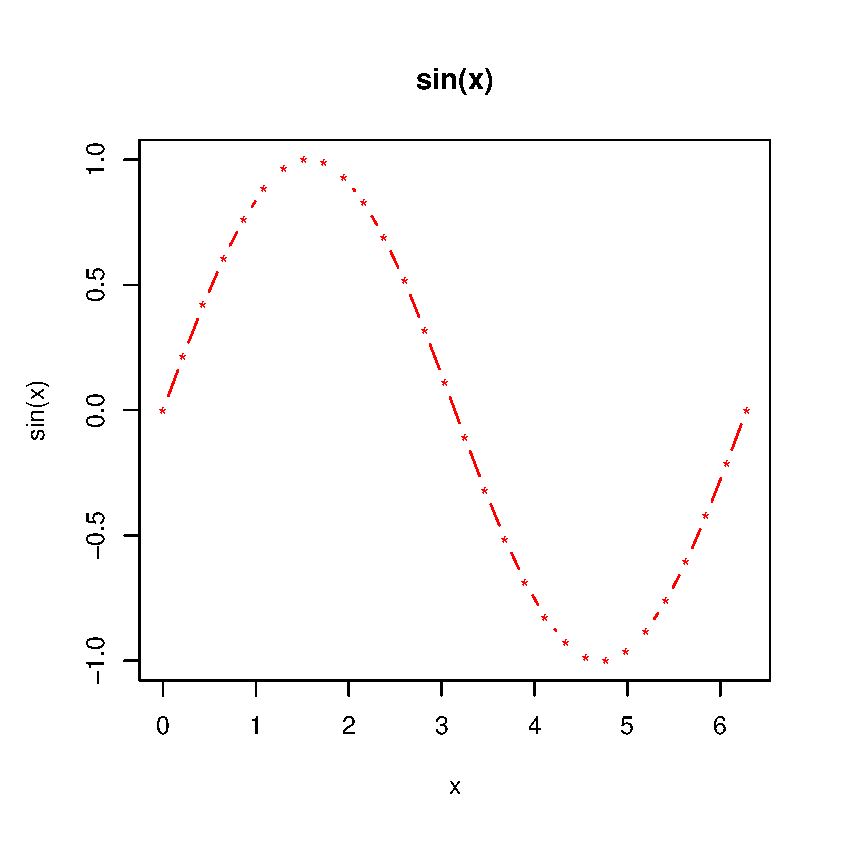
\includegraphics[width=3.0in]
{01Intro/RplotEx1.eps}
\end{center}
\caption{แบบฝึกหัด \texttt{plot} ข้อ 4}
\label{fig: R plot ex1}
\end{figure}
%

\paragraph{5.} จงศึกษาคำสั่ง \verb|par|, \verb|lines|, \verb|legend| และวาดกราฟดังแสดงในรูป~\ref{fig: R plot ex2}.
สังเกตุทั้งสองกราฟอยู่ในรูปเดียวกัน กราฟทางซ้ายมือแกน y มีค่าระหว่าง $-2$ ถึง $2$, ระบุชื่อของแกน y และ แกน x ตามรูป~\ref{fig: R plot ex2}.

%
\begin{figure}
\begin{center}
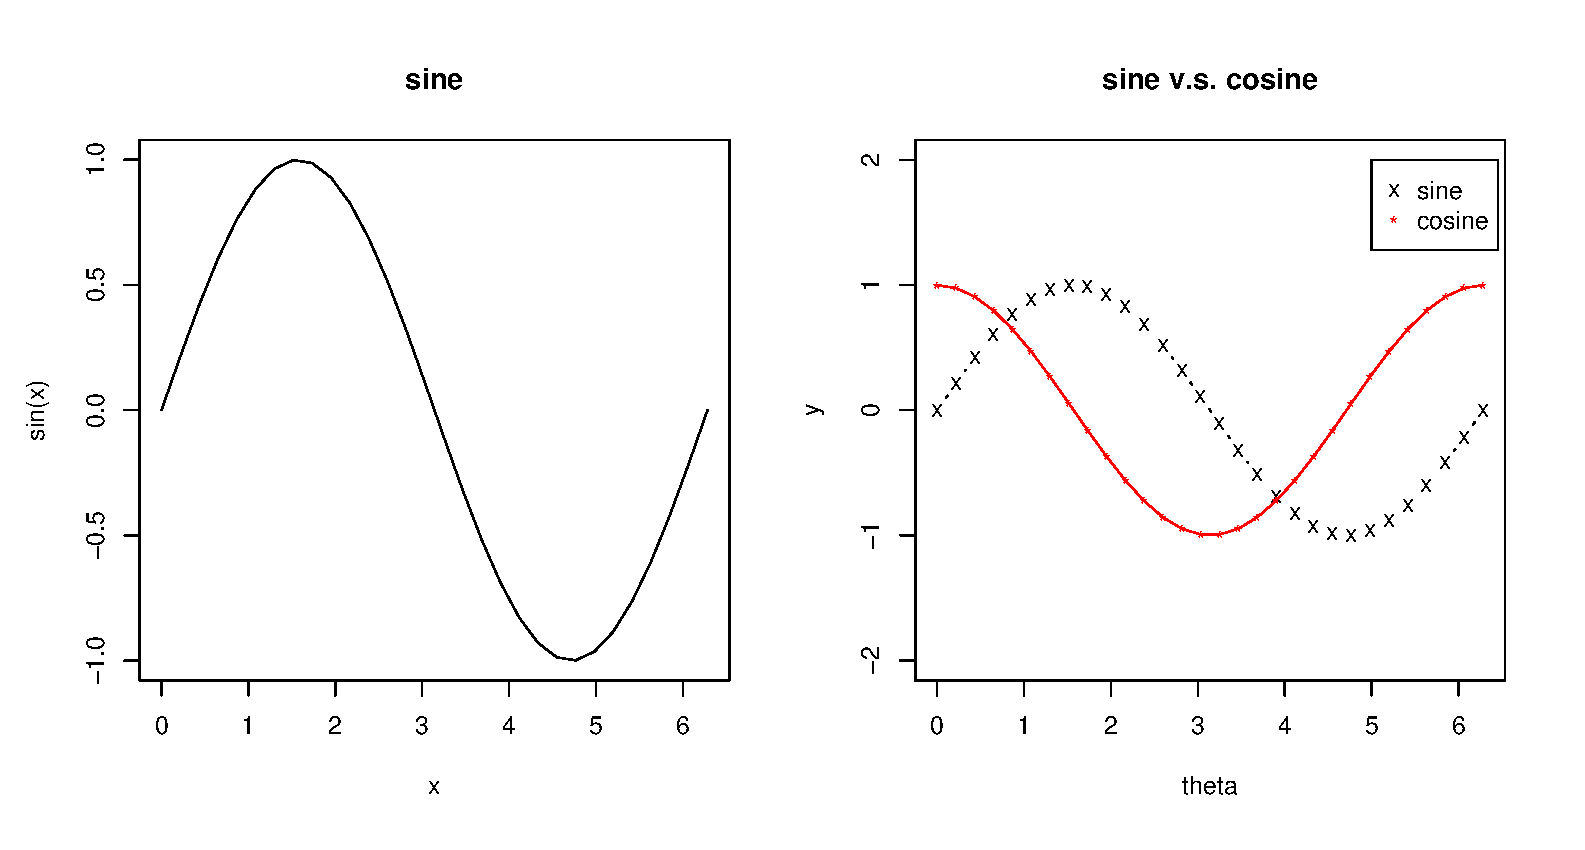
\includegraphics[width=6.0in]
{01Intro/RplotEx2.eps}
\end{center}
\caption{แบบฝึกหัด \texttt{plot} ข้อ 5}
\label{fig: R plot ex2}
\end{figure}
%

\paragraph{6.} โปรแกรมข้างล่างนี้ใช้วาดรูป~\ref{fig: R plot ex3}.
\begin{verbatim}
> x <- seq(0,100,len=5)
> plot(x, sin(x), type='l')
\end{verbatim}
จงวิเคราะห์และอธิบายว่าทำไมรูปที่ได้ไม่เห็นเป็นรูปโค้งขึ้นลงเหมือนรูปไซน์ที่คุ้นเคย.

%
\begin{figure}
\begin{center}
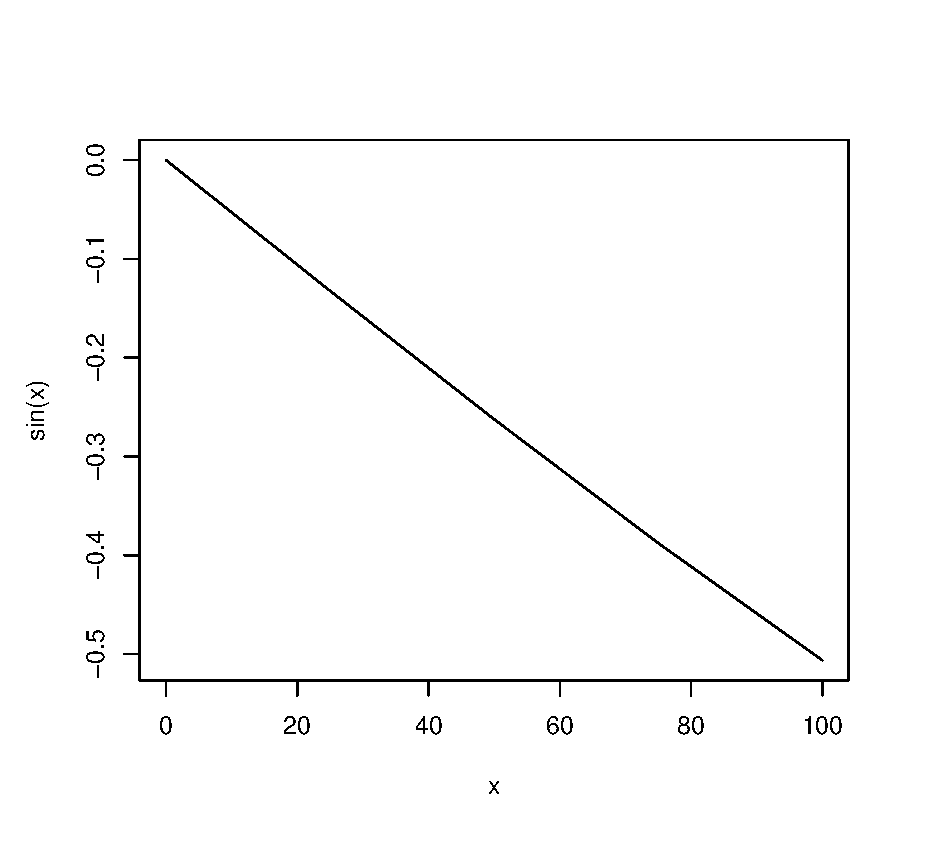
\includegraphics[width=3.0in]
{01Intro/RplotEx3.eps}
\end{center}
\caption{แบบฝึกหัดวิเคราะห์ข้อ 6}
\label{fig: R plot ex3}
\end{figure}
%

\paragraph{7.} โปรแกรมข้างล่างนี้ใช้วาดรูป~\ref{fig: R plot ex5}. 
\begin{lstlisting}[language=R,caption={โค้ดสำหรับรูปแบบฝึกหัดข้อ 7}]
x <- seq(-0.5, 0.5, len=50)

plot(x, 10*exp(-x^2)-8.8, type='l', ylab='y',
  main='10*exp(-x^2)-8.8 v.s. sin(x)')
lines(x, sin(x), col='red', lty=2)
legend(0, -0.5, c('10*exp(-x^2)-8.8', 'sin(x)'),
   lty=c(1,2), col=c('black', 'red'))
\end{lstlisting}
จงวิเคราะห์และอธิบายว่าทำไมกราฟเส้นประ ซึ่งเป็นกราฟของฟังชั่นไซน์จึงไม่เป็นรูปโค้งขึ้นลงเหมือนรูปไซน์ที่คุ้นเคย.

%
\begin{figure}
\begin{center}
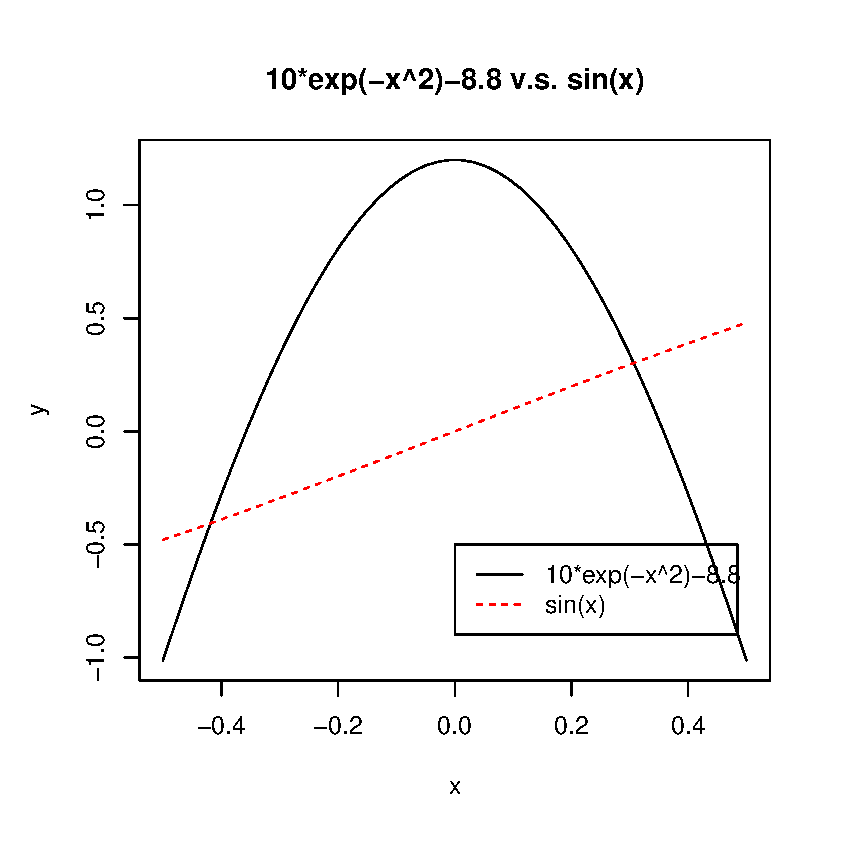
\includegraphics[width=3.0in]
{01Intro/RplotEx5.eps}
\end{center}
\caption{แบบฝึกหัดวิเคราะห์ข้อ 7}
\label{fig: R plot ex5}
\end{figure}
%

\paragraph{8.} จากโปรแกรมและผลการรันดังแสดงข้างล่างนี้
จงอภิปรายว่าทำไมมี $x$ บางตัวไม่เท่ากับ $7 \cdot y$ ซึ่ง $y = x/7$.
\begin{verbatim}
> x <- seq(1,10, len=20)
> y <- x/7
> x == 7*y
 [1]  TRUE  TRUE  TRUE  TRUE  TRUE  TRUE  TRUE  TRUE
 [9]  TRUE  TRUE  TRUE  TRUE  TRUE FALSE FALSE  TRUE
[17]  TRUE  TRUE  TRUE  TRUE
\end{verbatim}
จงวิเคราะห์และอธิบายผลของ \verb|x == 7*(x/7)| กับ \verb|x == 7*x/7| ประกอบ
พร้อมอภิปรายการประยุกต์ใช้ประเด็นที่ได้เรียนรู้นี้กับสถานการณ์ที่อาจจะเกิดขึ้น รวมถึงความเสี่ยงและโอกาส.

\paragraph{9.} %%จากคณิตศาสตร์ $\log( \exp(x) ) = x$ และ $\log(A/B) = \log(A) - \log(B)$, 
โปรแกรมข้างล่างนี้วาดรูป~\ref{fig: R plot ex6}.
\lstinputlisting[language=R,caption={โปรแกรมสำหรับรูปแบบฝึกหัดข้อ 9}]{01Intro/introQ9Code.r}

รูปบนเป็นกราฟของ $x^2$ (เส้นทึบสีดำ) และ $x^2 - x^2$ (เส้นประสีแดง).
รูปล่างเป็นกราฟของ $\log(\exp(x^2))$ (เส้นทึบสีดำ) และ $\log(\exp(x^2)/\exp(x^2))$ (เส้นประสีแดง).
จากความรู้คณิตศาสตร์ จะได้ $\log(\exp(x^2)) = x^2$ และ $\log(\exp(x^2)/\exp(x^2)) = x^2 - x^2$ 
แต่ทำไมกราฟรูปบนจึงต่างจากรูปล่าง (รูปบนแสดงค่าไปจนถึง $x = 30$ แต่รูปล่างไม่ถึง). 
จงอภิปราย.

%
\begin{figure}
\begin{center}
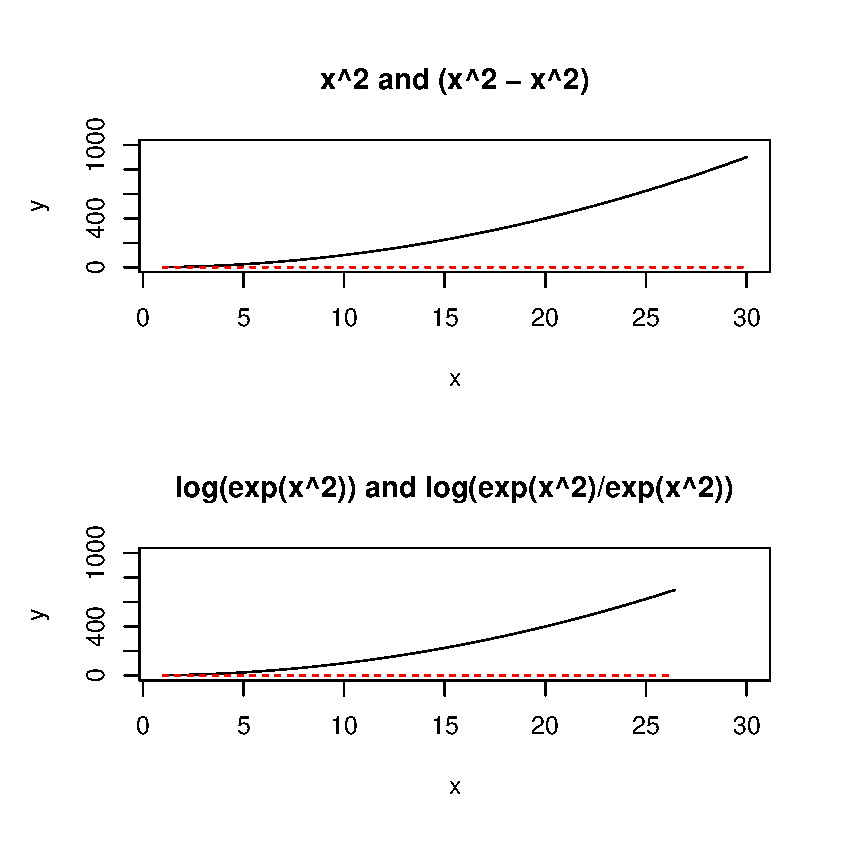
\includegraphics[width=4.0in]
{01Intro/RplotEx6.eps}
\end{center}
\caption{แบบฝึกหัดวิเคราะห์ข้อ 9}
\label{fig: R plot ex6}
\end{figure}
%

\paragraph{10.} จงศึกษาผลจากการคูณกันของเวกเตอร์ทิศทางต่างๆ.
จากโปรแกรมอาร์โปรเจคข้างล่าง ทดลองดูผลการคูณกันของเวกเตอร์ $2$ เวกเตอร์
นั่นคือ \verb|vq1| กับ \verb|v2|
โดย \verb|vq1| จะอยู่ที่เดิม แต่ \verb|v2| จะเปลี่ยนทิศทางไป ($20$ ค่ารอบทิศทาง ตั้งแต่ $\frac{1}{10}\pi$ จนถึง $2 \pi$).
โปรแกรมจะวาดรูปออกมา $2$ รูป 
แต่ละรูปแสดง $10$ ภาพย่อย
รวมทั้งหมด $20$ ภาพย่อย (แต่ละภาพย่อยแทนแต่ละทิศทางของ \verb|v2|).
สังเกตุผลจากการคูณ ที่ระบุไว้ในแต่ละภาพ และทดลองเปลี่ยนค่าองศาของ \verb|vq1| ให้เป็นค่าอื่นๆ (เปลี่ยนค่าของ \verb|theta1| ที่ตอนนี้ระบุเป็น \verb|6*pi/10|)
สรุปผลจากการคูณเวกเตอร์ทิศทางต่างๆ และตอบคำถาม ก.-จ. (เวกเตอร์ทุกตัวมีขนาดมากกว่า $0$)
\lstinputlisting[language=R,caption={โปรแกรมวาดรูปสำหรับแบบฝึกหัดข้อ 10}]{01Intro/introQ10Code.r}


\begin{itemize}
\item ก. ถ้าเวกเตอร์ A คูณกับเวกเตอร์ B ได้ผลเป็นบวก และเวกเตอร์ A ชี้ไปทิศทางสองนาฬิกา (เทียบเท่า $30$ องศาจากแกน $x$) สิ่งนี้บอกอะไรได้บ้างเกี่ยวกับทิศทางของเวกเตอร์ B

\item ข. ถ้าเวกเตอร์ A จากข้อ ก. ขนานกับเวกเตอร์ C ผลคูณของเวกเตอร์ A กับ C ผลคูณนี้จะเป็นอะไรได้บ้าง และเป็นอะไรไม่ได้บ้าง

\item ค. ถ้าเวกเตอร์ A จากข้อ ก. ตั้งฉากกับเวกเตอร์ D ผลคูณของเวกเตอร์ A กับ D ผลคูณนี้จะเป็นอะไรได้บ้าง และเป็นอะไรไม่ได้บ้าง

\item ง. ถ้าเวกเตอร์ A จากข้อ ก. คูณกับเวกเตอร์ E ได้ผลเป็นลบ
สิ่งนี้บอกอะไรได้บ้างเกี่ยวกับทิศทางของเวกเตอร์ E

\item จ. ถ้าหากต้องการผลคูณเวกเตอร์ A จากข้อ ก. กับเวกเตอร์ F ให้ได้ผลเป็นบวกและมีค่ามากที่สุด เวกเตอร์ F ควรมีทิศทางอย่างไร
\end{itemize}

